\begin{figure}
\centering
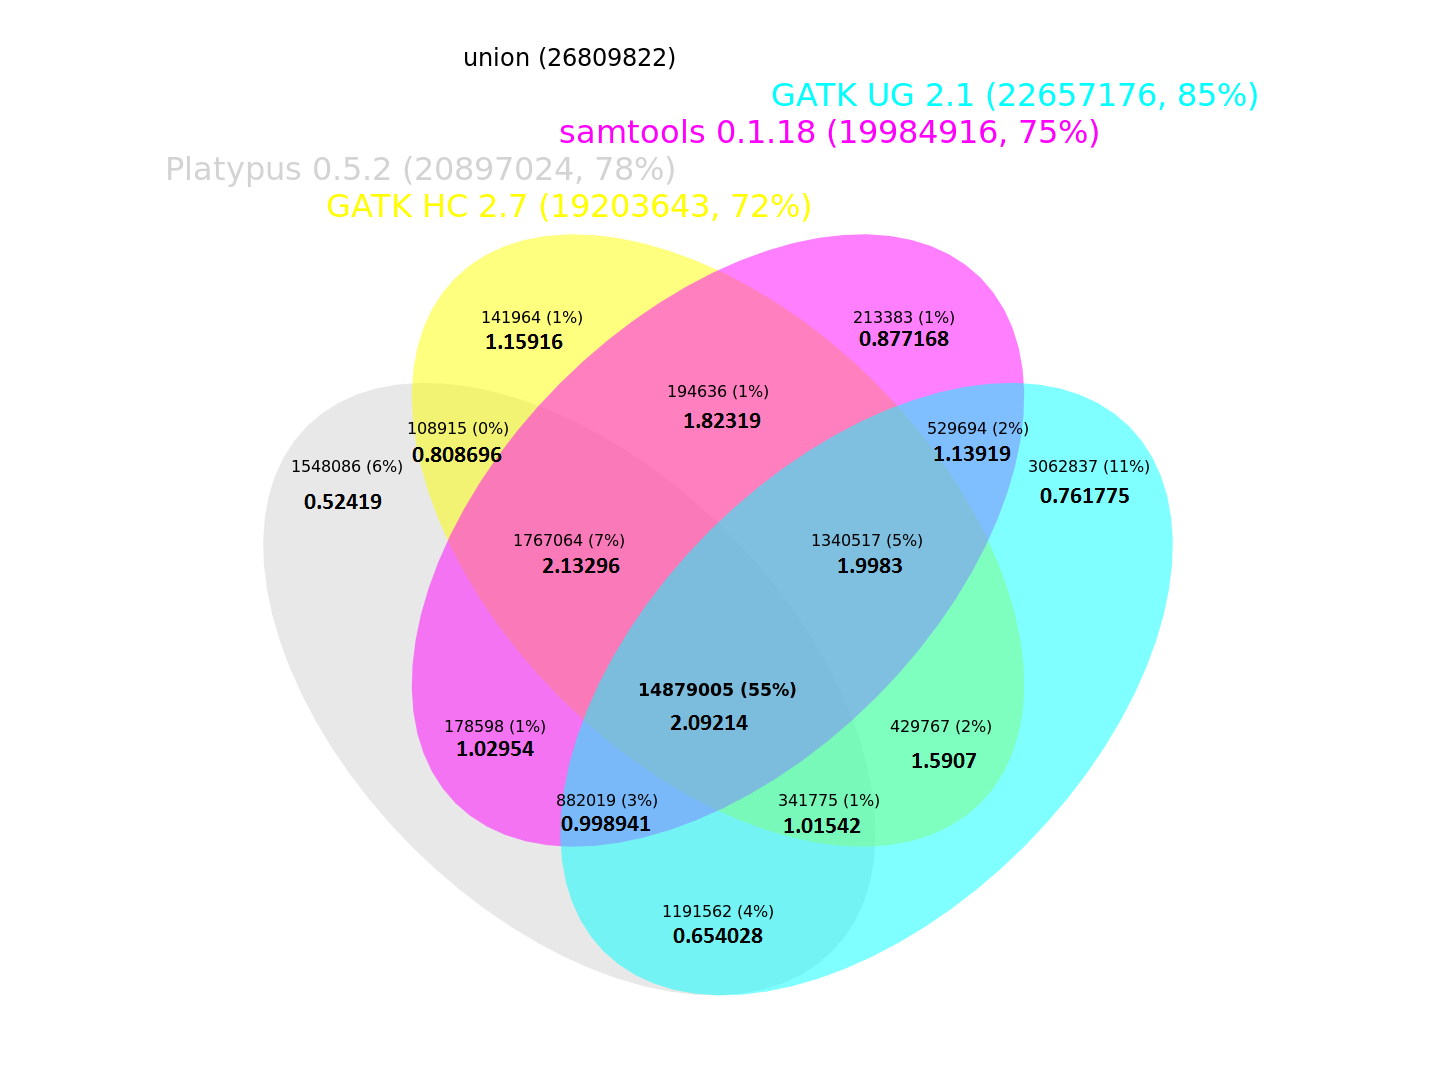
\includegraphics{Chapter2/fig/venn4_varcall_Platypus_filter_QUAL4_incl_MNPs_TiTv}
\caption{Comparison of variant callers. SNPs and MNPs were called with four different variant callers from Baganda 4x sequence data. A quality threshold of 4 was applied. The small numbers show the count of variants in each Venn set and the size of each set as a percentage of the size of the union set is printed in a parenthesis. The larger number in bold is the Ti/Tv ratio in each set. Platypus has a high sensitivity comapred to the union set, but the variants unique to Platypus have a low Ti/Tv ratio, which indicates that they are false positives. \gls{GATK} \gls{UG} despite having a great number of unique variants has a higher Ti/Tv ratio than Platypus.}
\label{fig:venn4_varcall_Platypus_filter_QUAL4_incl_MNPs_TiTv}
\end{figure}